\documentclass[1p]{elsarticle_modified}
%\bibliographystyle{elsarticle-num}

%\usepackage[colorlinks]{hyperref}
%\usepackage{abbrmath_seonhwa} %\Abb, \Ascr, \Acal ,\Abf, \Afrak
\usepackage{amsfonts}
\usepackage{amssymb}
\usepackage{amsmath}
\usepackage{amsthm}
\usepackage{scalefnt}
\usepackage{amsbsy}
\usepackage{kotex}
\usepackage{caption}
\usepackage{subfig}
\usepackage{color}
\usepackage{graphicx}
\usepackage{xcolor} %% white, black, red, green, blue, cyan, magenta, yellow
\usepackage{float}
\usepackage{setspace}
\usepackage{hyperref}

\usepackage{tikz}
\usetikzlibrary{arrows}

\usepackage{multirow}
\usepackage{array} % fixed length table
\usepackage{hhline}

%%%%%%%%%%%%%%%%%%%%%
\makeatletter
\renewcommand*\env@matrix[1][\arraystretch]{%
	\edef\arraystretch{#1}%
	\hskip -\arraycolsep
	\let\@ifnextchar\new@ifnextchar
	\array{*\c@MaxMatrixCols c}}
\makeatother %https://tex.stackexchange.com/questions/14071/how-can-i-increase-the-line-spacing-in-a-matrix
%%%%%%%%%%%%%%%

\usepackage[normalem]{ulem}

\newcommand{\msout}[1]{\ifmmode\text{\sout{\ensuremath{#1}}}\else\sout{#1}\fi}
%SOURCE: \msout is \stkout macro in https://tex.stackexchange.com/questions/20609/strikeout-in-math-mode

\newcommand{\cancel}[1]{
	\ifmmode
	{\color{red}\msout{#1}}
	\else
	{\color{red}\sout{#1}}
	\fi
}

\newcommand{\add}[1]{
	{\color{blue}\uwave{#1}}
}

\newcommand{\replace}[2]{
	\ifmmode
	{\color{red}\msout{#1}}{\color{blue}\uwave{#2}}
	\else
	{\color{red}\sout{#1}}{\color{blue}\uwave{#2}}
	\fi
}

\newcommand{\Sol}{\mathcal{S}} %segment
\newcommand{\D}{D} %diagram
\newcommand{\A}{\mathcal{A}} %arc


%%%%%%%%%%%%%%%%%%%%%%%%%%%%%5 test

\def\sl{\operatorname{\textup{SL}}(2,\Cbb)}
\def\psl{\operatorname{\textup{PSL}}(2,\Cbb)}
\def\quan{\mkern 1mu \triangleright \mkern 1mu}

\theoremstyle{definition}
\newtheorem{thm}{Theorem}[section]
\newtheorem{prop}[thm]{Proposition}
\newtheorem{lem}[thm]{Lemma}
\newtheorem{ques}[thm]{Question}
\newtheorem{cor}[thm]{Corollary}
\newtheorem{defn}[thm]{Definition}
\newtheorem{exam}[thm]{Example}
\newtheorem{rmk}[thm]{Remark}
\newtheorem{alg}[thm]{Algorithm}

\newcommand{\I}{\sqrt{-1}}
\begin{document}

%\begin{frontmatter}
%
%\title{Boundary parabolic representations of knots up to 8 crossings}
%
%%% Group authors per affiliation:
%\author{Yunhi Cho} 
%\address{Department of Mathematics, University of Seoul, Seoul, Korea}
%\ead{yhcho@uos.ac.kr}
%
%
%\author{Seonhwa Kim} %\fnref{s_kim}}
%\address{Center for Geometry and Physics, Institute for Basic Science, Pohang, 37673, Korea}
%\ead{ryeona17@ibs.re.kr}
%
%\author{Hyuk Kim}
%\address{Department of Mathematical Sciences, Seoul National University, Seoul 08826, Korea}
%\ead{hyukkim@snu.ac.kr}
%
%\author{Seokbeom Yoon}
%\address{Department of Mathematical Sciences, Seoul National University, Seoul, 08826,  Korea}
%\ead{sbyoon15@snu.ac.kr}
%
%\begin{abstract}
%We find all boundary parabolic representation of knots up to 8 crossings.
%
%\end{abstract}
%\begin{keyword}
%    \MSC[2010] 57M25 
%\end{keyword}
%
%\end{frontmatter}

%\linenumbers
%\tableofcontents
%
\newcommand\colored[1]{\textcolor{white}{\rule[-0.35ex]{0.8em}{1.4ex}}\kern-0.8em\color{red} #1}%
%\newcommand\colored[1]{\textcolor{white}{ #1}\kern-2.17ex	\textcolor{white}{ #1}\kern-1.81ex	\textcolor{white}{ #1}\kern-2.15ex\color{red}#1	}

{\Large $\underline{12n_{0456}~(K12n_{0456})}$}

\setlength{\tabcolsep}{10pt}
\renewcommand{\arraystretch}{1.6}
\vspace{1cm}\begin{tabular}{m{100pt}>{\centering\arraybackslash}m{274pt}}
\multirow{5}{120pt}{
	\centering
	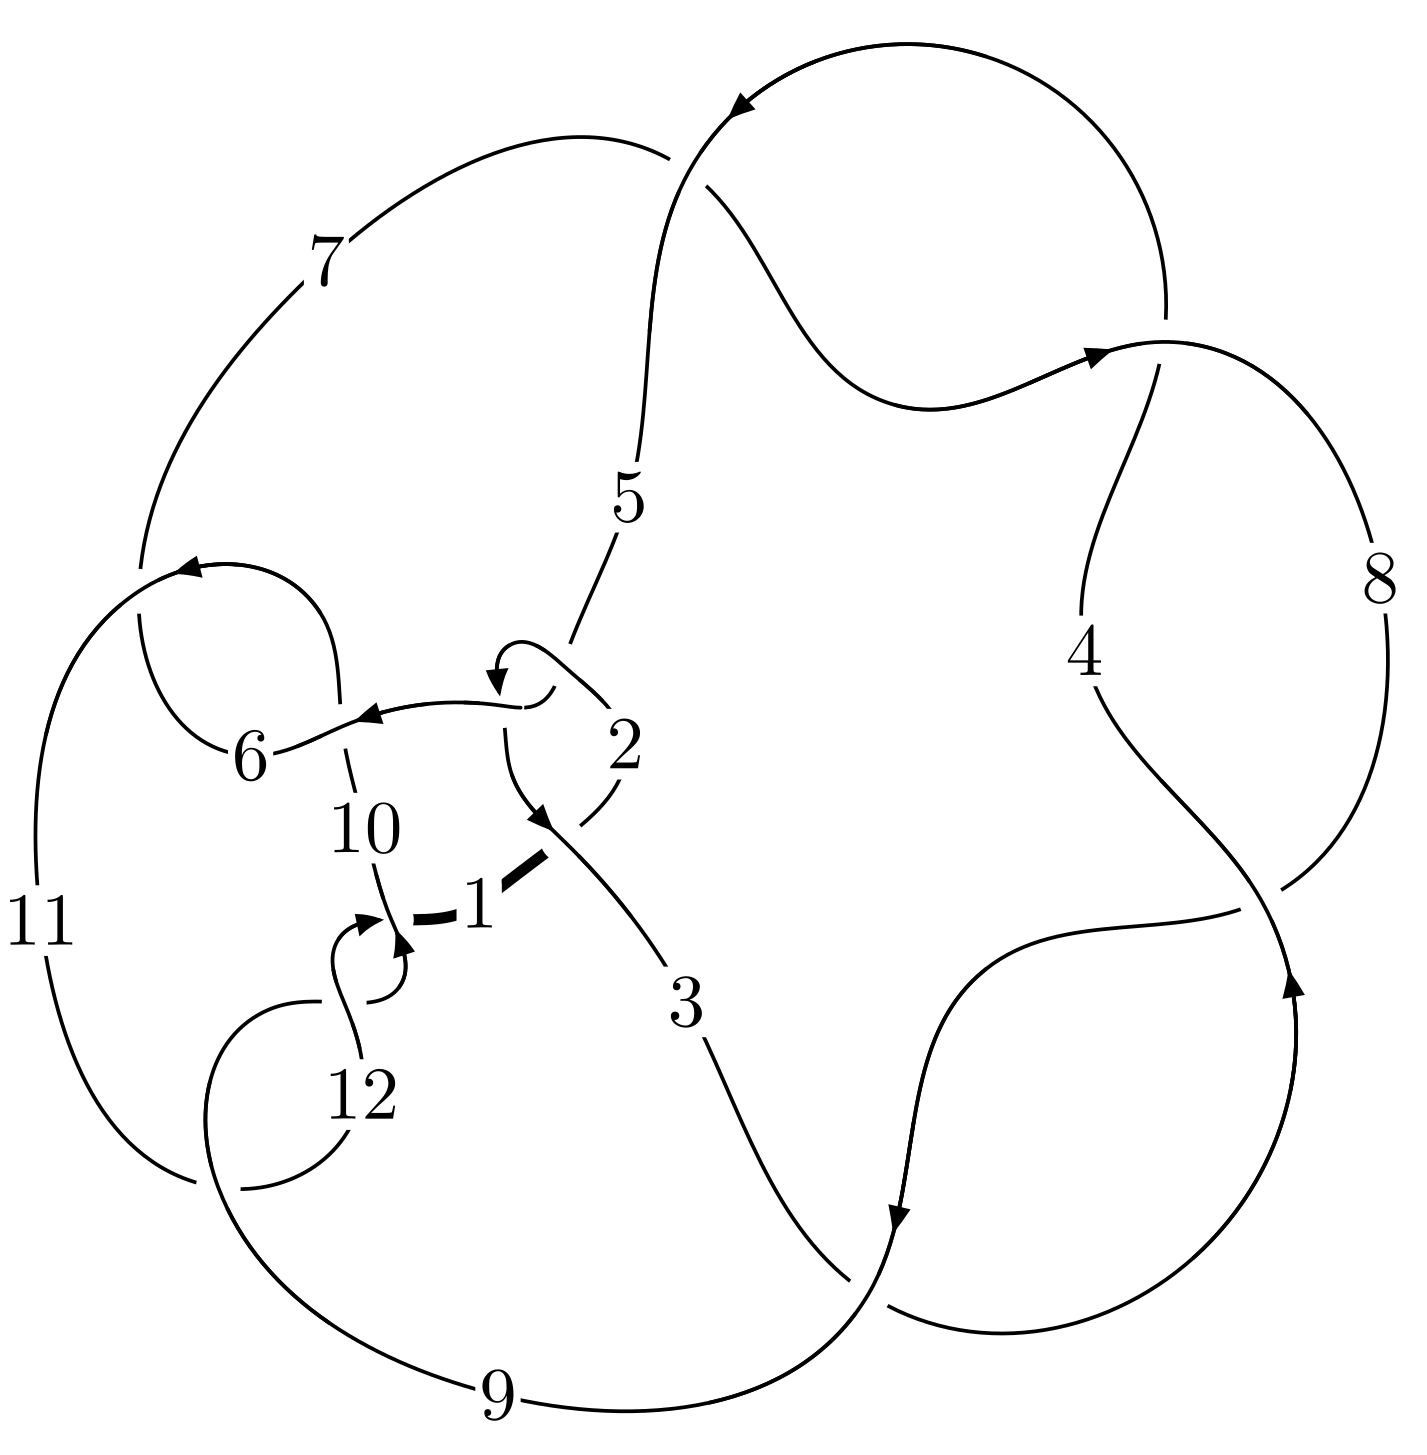
\includegraphics[width=112pt]{../../../GIT/diagram.site/Diagrams/png/2545_12n_0456.png}\\
\ \ \ A knot diagram\footnotemark}&
\allowdisplaybreaks
\textbf{Linearized knot diagam} \\
\cline{2-2}
 &
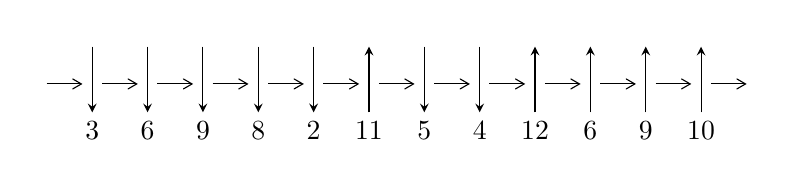
\begin{tikzpicture}[x=20pt, y=17pt]
	% nodes
	\node (C0) at (0, 0) {};
	\node (C1) at (1, 0) {};
	\node (C1U) at (1, +1) {};
	\node (C1D) at (1, -1) {3};

	\node (C2) at (2, 0) {};
	\node (C2U) at (2, +1) {};
	\node (C2D) at (2, -1) {6};

	\node (C3) at (3, 0) {};
	\node (C3U) at (3, +1) {};
	\node (C3D) at (3, -1) {9};

	\node (C4) at (4, 0) {};
	\node (C4U) at (4, +1) {};
	\node (C4D) at (4, -1) {8};

	\node (C5) at (5, 0) {};
	\node (C5U) at (5, +1) {};
	\node (C5D) at (5, -1) {2};

	\node (C6) at (6, 0) {};
	\node (C6U) at (6, +1) {};
	\node (C6D) at (6, -1) {11};

	\node (C7) at (7, 0) {};
	\node (C7U) at (7, +1) {};
	\node (C7D) at (7, -1) {5};

	\node (C8) at (8, 0) {};
	\node (C8U) at (8, +1) {};
	\node (C8D) at (8, -1) {4};

	\node (C9) at (9, 0) {};
	\node (C9U) at (9, +1) {};
	\node (C9D) at (9, -1) {12};

	\node (C10) at (10, 0) {};
	\node (C10U) at (10, +1) {};
	\node (C10D) at (10, -1) {6};

	\node (C11) at (11, 0) {};
	\node (C11U) at (11, +1) {};
	\node (C11D) at (11, -1) {9};

	\node (C12) at (12, 0) {};
	\node (C12U) at (12, +1) {};
	\node (C12D) at (12, -1) {10};
	\node (C13) at (13, 0) {};

	% arrows
	\draw[->,>={angle 60}]
	(C0) edge (C1) (C1) edge (C2) (C2) edge (C3) (C3) edge (C4) (C4) edge (C5) (C5) edge (C6) (C6) edge (C7) (C7) edge (C8) (C8) edge (C9) (C9) edge (C10) (C10) edge (C11) (C11) edge (C12) (C12) edge (C13) ;	\draw[->,>=stealth]
	(C1U) edge (C1D) (C2U) edge (C2D) (C3U) edge (C3D) (C4U) edge (C4D) (C5U) edge (C5D) (C6D) edge (C6U) (C7U) edge (C7D) (C8U) edge (C8D) (C9D) edge (C9U) (C10D) edge (C10U) (C11D) edge (C11U) (C12D) edge (C12U) ;
	\end{tikzpicture} \\
\hhline{~~} \\& 
\textbf{Solving Sequence} \\ \cline{2-2} 
 &
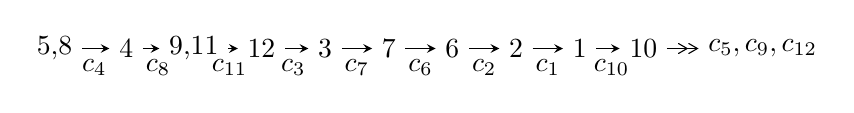
\begin{tikzpicture}[x=23pt, y=7pt]
	% node
	\node (A0) at (-1/8, 0) {5,8};
	\node (A1) at (1, 0) {4};
	\node (A2) at (33/16, 0) {9,11};
	\node (A3) at (25/8, 0) {12};
	\node (A4) at (33/8, 0) {3};
	\node (A5) at (41/8, 0) {7};
	\node (A6) at (49/8, 0) {6};
	\node (A7) at (57/8, 0) {2};
	\node (A8) at (65/8, 0) {1};
	\node (A9) at (73/8, 0) {10};
	\node (C1) at (1/2, -1) {$c_{4}$};
	\node (C2) at (3/2, -1) {$c_{8}$};
	\node (C3) at (21/8, -1) {$c_{11}$};
	\node (C4) at (29/8, -1) {$c_{3}$};
	\node (C5) at (37/8, -1) {$c_{7}$};
	\node (C6) at (45/8, -1) {$c_{6}$};
	\node (C7) at (53/8, -1) {$c_{2}$};
	\node (C8) at (61/8, -1) {$c_{1}$};
	\node (C9) at (69/8, -1) {$c_{10}$};
	\node (A10) at (11, 0) {$c_{5},c_{9},c_{12}$};

	% edge
	\draw[->,>=stealth]	
	(A0) edge (A1) (A1) edge (A2) (A2) edge (A3) (A3) edge (A4) (A4) edge (A5) (A5) edge (A6) (A6) edge (A7) (A7) edge (A8) (A8) edge (A9) ;
	\draw[->>,>={angle 60}]	
	(A9) edge (A10);
\end{tikzpicture} \\ 

\end{tabular} \\

\footnotetext{
The image of knot diagram is generated by the software ``\textbf{Draw programme}" developed by Andrew Bartholomew(\url{http://www.layer8.co.uk/maths/draw/index.htm\#Running-draw}), where we modified some parts for our purpose(\url{https://github.com/CATsTAILs/LinksPainter}).
}\phantom \\ \newline 
\centering \textbf{Ideals for irreducible components\footnotemark of $X_{\text{par}}$} 
 
\begin{align*}
I^u_{1}&=\langle 
6263646729160 u^{18}+14140809413971 u^{17}+\cdots+89100980340036 b-30737815843748,\\
\phantom{I^u_{1}}&\phantom{= \langle  }18590835030469 u^{18}+42781634933956 u^{17}+\cdots+89100980340036 a+3563580716326,\\
\phantom{I^u_{1}}&\phantom{= \langle  }u^{19}+2 u^{18}+\cdots-4 u+4\rangle \\
I^u_{2}&=\langle 
-2 u^4+3 u^3-8 u^2+3 b+7 u-5,\;-2 u^4+3 u^3-8 u^2+3 a+7 u-5,\;u^5- u^4+4 u^3-3 u^2+3 u-1\rangle \\
I^u_{3}&=\langle 
a u+3 b-4 a-2 u-1,\;2 a^2+3 a u-2 a+u-3,\;u^2+2\rangle \\
\\
I^v_{1}&=\langle 
a,\;b- v+2,\;v^2-3 v+1\rangle \\
\end{align*}
\raggedright * 4 irreducible components of $\dim_{\mathbb{C}}=0$, with total 30 representations.\\
\footnotetext{All coefficients of polynomials are rational numbers. But the coefficients are sometimes approximated in decimal forms when there is not enough margin.}
\newpage
\renewcommand{\arraystretch}{1}
\centering \section*{I. $I^u_{1}= \langle 6.26\times10^{12} u^{18}+1.41\times10^{13} u^{17}+\cdots+8.91\times10^{13} b-3.07\times10^{13},\;1.86\times10^{13} u^{18}+4.28\times10^{13} u^{17}+\cdots+8.91\times10^{13} a+3.56\times10^{12},\;u^{19}+2 u^{18}+\cdots-4 u+4 \rangle$}
\flushleft \textbf{(i) Arc colorings}\\
\begin{tabular}{m{7pt} m{180pt} m{7pt} m{180pt} }
\flushright $a_{5}=$&$\begin{pmatrix}1\\0\end{pmatrix}$ \\
\flushright $a_{8}=$&$\begin{pmatrix}0\\u\end{pmatrix}$ \\
\flushright $a_{4}=$&$\begin{pmatrix}1\\- u^2\end{pmatrix}$ \\
\flushright $a_{9}=$&$\begin{pmatrix}- u\\u^3+u\end{pmatrix}$ \\
\flushright $a_{11}=$&$\begin{pmatrix}-0.208649 u^{18}-0.480148 u^{17}+\cdots+3.87234 u-0.0399949\\-0.0702983 u^{18}-0.158705 u^{17}+\cdots+2.22000 u+0.344977\end{pmatrix}$ \\
\flushright $a_{12}=$&$\begin{pmatrix}-0.244992 u^{18}-0.555084 u^{17}+\cdots+4.64401 u+0.313303\\-0.0108279 u^{18}-0.00284769 u^{17}+\cdots+1.31196 u-0.0173194\end{pmatrix}$ \\
\flushright $a_{3}=$&$\begin{pmatrix}u^2+1\\- u^4-2 u^2\end{pmatrix}$ \\
\flushright $a_{7}=$&$\begin{pmatrix}u\\u\end{pmatrix}$ \\
\flushright $a_{6}=$&$\begin{pmatrix}-0.224318 u^{18}-0.601824 u^{17}+\cdots+0.750211 u+2.25690\\0.0287859 u^{18}+0.0720971 u^{17}+\cdots+0.834764 u+0.0468869\end{pmatrix}$ \\
\flushright $a_{2}=$&$\begin{pmatrix}-0.274839 u^{18}-0.716004 u^{17}+\cdots+1.86949 u+2.91655\\0.135398 u^{18}+0.314325 u^{17}+\cdots-1.55333 u-1.32495\end{pmatrix}$ \\
\flushright $a_{1}=$&$\begin{pmatrix}-0.328521 u^{18}-0.867710 u^{17}+\cdots+1.09177 u+2.92776\\0.181013 u^{18}+0.450207 u^{17}+\cdots-1.64773 u-1.56042\end{pmatrix}$ \\
\flushright $a_{10}=$&$\begin{pmatrix}0.265765 u^{18}+0.718930 u^{17}+\cdots+0.293501 u-3.20338\\-0.180775 u^{18}-0.461139 u^{17}+\cdots+2.62586 u+1.11854\end{pmatrix}$\\&\end{tabular}
\flushleft \textbf{(ii) Obstruction class $= -1$}\\~\\
\flushleft \textbf{(iii) Cusp Shapes $= \frac{71570433112501}{66825735255027} u^{18}+\frac{150381276390913}{66825735255027} u^{17}+\cdots-\frac{2412887014500530}{66825735255027} u-\frac{508458695878388}{66825735255027}$}\\~\\
\newpage\renewcommand{\arraystretch}{1}
\flushleft \textbf{(iv) u-Polynomials at the component}\newline \\
\begin{tabular}{m{50pt}|m{274pt}}
Crossings & \hspace{64pt}u-Polynomials at each crossing \\
\hline $$\begin{aligned}c_{1}\end{aligned}$$&$\begin{aligned}
&u^{19}+26 u^{18}+\cdots+17485 u+361
\end{aligned}$\\
\hline $$\begin{aligned}c_{2},c_{5}\end{aligned}$$&$\begin{aligned}
&u^{19}+4 u^{18}+\cdots-105 u-19
\end{aligned}$\\
\hline $$\begin{aligned}c_{3},c_{4},c_{7}\\c_{8}\end{aligned}$$&$\begin{aligned}
&u^{19}-2 u^{18}+\cdots-4 u-4
\end{aligned}$\\
\hline $$\begin{aligned}c_{6},c_{10}\end{aligned}$$&$\begin{aligned}
&u^{19}+2 u^{18}+\cdots-384 u-288
\end{aligned}$\\
\hline $$\begin{aligned}c_{9},c_{11},c_{12}\end{aligned}$$&$\begin{aligned}
&u^{19}+9 u^{18}+\cdots-48 u+9
\end{aligned}$\\
\hline
\end{tabular}\\~\\
\newpage\renewcommand{\arraystretch}{1}
\flushleft \textbf{(v) Riley Polynomials at the component}\newline \\
\begin{tabular}{m{50pt}|m{274pt}}
Crossings & \hspace{64pt}Riley Polynomials at each crossing \\
\hline $$\begin{aligned}c_{1}\end{aligned}$$&$\begin{aligned}
&y^{19}-58 y^{18}+\cdots+218537949 y-130321
\end{aligned}$\\
\hline $$\begin{aligned}c_{2},c_{5}\end{aligned}$$&$\begin{aligned}
&y^{19}-26 y^{18}+\cdots+17485 y-361
\end{aligned}$\\
\hline $$\begin{aligned}c_{3},c_{4},c_{7}\\c_{8}\end{aligned}$$&$\begin{aligned}
&y^{19}+16 y^{18}+\cdots+336 y-16
\end{aligned}$\\
\hline $$\begin{aligned}c_{6},c_{10}\end{aligned}$$&$\begin{aligned}
&y^{19}+24 y^{18}+\cdots+1101312 y-82944
\end{aligned}$\\
\hline $$\begin{aligned}c_{9},c_{11},c_{12}\end{aligned}$$&$\begin{aligned}
&y^{19}-5 y^{18}+\cdots+3042 y-81
\end{aligned}$\\
\hline
\end{tabular}\\~\\
\newpage\flushleft \textbf{(vi) Complex Volumes and Cusp Shapes}
$$\begin{array}{c|c|c}  
\text{Solutions to }I^u_{1}& \I (\text{vol} + \sqrt{-1}CS) & \text{Cusp shape}\\
 \hline 
\begin{aligned}
u &= -0.074260 + 0.917453 I \\
a &= -0.994466 - 0.538689 I \\
b &= -0.317235 + 0.013665 I\end{aligned}
 & \phantom{-}1.53865 - 1.34534 I & \phantom{-}0.43995 + 3.44940 I \\ \hline\begin{aligned}
u &= -0.074260 - 0.917453 I \\
a &= -0.994466 + 0.538689 I \\
b &= -0.317235 - 0.013665 I\end{aligned}
 & \phantom{-}1.53865 + 1.34534 I & \phantom{-}0.43995 - 3.44940 I \\ \hline\begin{aligned}
u &= \phantom{-}0.682490 + 0.464817 I \\
a &= -0.506827 + 0.094261 I \\
b &= \phantom{-}0.670269 - 1.079920 I\end{aligned}
 & -1.35153 - 0.43293 I & -1.33817 + 2.53322 I \\ \hline\begin{aligned}
u &= \phantom{-}0.682490 - 0.464817 I \\
a &= -0.506827 - 0.094261 I \\
b &= \phantom{-}0.670269 + 1.079920 I\end{aligned}
 & -1.35153 + 0.43293 I & -1.33817 - 2.53322 I \\ \hline\begin{aligned}
u &= \phantom{-}0.017361 + 1.304010 I \\
a &= \phantom{-}1.72921 - 0.99084 I \\
b &= \phantom{-}1.41667 - 1.52874 I\end{aligned}
 & \phantom{-}4.96292 + 0.91602 I & \phantom{-}7.77670 - 1.28958 I \\ \hline\begin{aligned}
u &= \phantom{-}0.017361 - 1.304010 I \\
a &= \phantom{-}1.72921 + 0.99084 I \\
b &= \phantom{-}1.41667 + 1.52874 I\end{aligned}
 & \phantom{-}4.96292 - 0.91602 I & \phantom{-}7.77670 + 1.28958 I \\ \hline\begin{aligned}
u &= -1.302620 + 0.369270 I \\
a &= \phantom{-}0.245431 - 0.163795 I \\
b &= \phantom{-}0.25437 + 1.92922 I\end{aligned}
 & -11.99340 + 5.23790 I & -1.08128 - 2.47083 I \\ \hline\begin{aligned}
u &= -1.302620 - 0.369270 I \\
a &= \phantom{-}0.245431 + 0.163795 I \\
b &= \phantom{-}0.25437 - 1.92922 I\end{aligned}
 & -11.99340 - 5.23790 I & -1.08128 + 2.47083 I \\ \hline\begin{aligned}
u &= \phantom{-}0.537549\phantom{ +0.000000I} \\
a &= -2.91204\phantom{ +0.000000I} \\
b &= \phantom{-}0.537401\phantom{ +0.000000I}\end{aligned}
 & \phantom{-}6.81454\phantom{ +0.000000I} & -5.63570\phantom{ +0.000000I} \\ \hline\begin{aligned}
u &= \phantom{-}0.58466 + 1.34467 I \\
a &= \phantom{-}0.940809 - 0.609725 I \\
b &= -0.099480 - 1.008040 I\end{aligned}
 & \phantom{-}1.61779 - 4.70658 I & \phantom{-}1.34919 + 3.92901 I\\
 \hline 
 \end{array}$$\newpage$$\begin{array}{c|c|c}  
\text{Solutions to }I^u_{1}& \I (\text{vol} + \sqrt{-1}CS) & \text{Cusp shape}\\
 \hline 
\begin{aligned}
u &= \phantom{-}0.58466 - 1.34467 I \\
a &= \phantom{-}0.940809 + 0.609725 I \\
b &= -0.099480 + 1.008040 I\end{aligned}
 & \phantom{-}1.61779 + 4.70658 I & \phantom{-}1.34919 - 3.92901 I \\ \hline\begin{aligned}
u &= -0.88316 + 1.34583 I \\
a &= \phantom{-}0.905620 + 0.537079 I \\
b &= -0.13821 + 1.90748 I\end{aligned}
 & -9.13960 + 2.40553 I & -0.343243 - 1.215158 I \\ \hline\begin{aligned}
u &= -0.88316 - 1.34583 I \\
a &= \phantom{-}0.905620 - 0.537079 I \\
b &= -0.13821 - 1.90748 I\end{aligned}
 & -9.13960 - 2.40553 I & -0.343243 + 1.215158 I \\ \hline\begin{aligned}
u &= \phantom{-}0.360199\phantom{ +0.000000I} \\
a &= -0.304748\phantom{ +0.000000I} \\
b &= \phantom{-}0.772322\phantom{ +0.000000I}\end{aligned}
 & -1.03641\phantom{ +0.000000I} & -12.4460\phantom{ +0.000000I} \\ \hline\begin{aligned}
u &= \phantom{-}0.13765 + 1.63790 I \\
a &= -0.009641 - 0.326348 I \\
b &= -0.387996 + 0.243197 I\end{aligned}
 & \phantom{-}13.18610 - 2.66860 I & \phantom{-}6.26035 - 0.13482 I \\ \hline\begin{aligned}
u &= \phantom{-}0.13765 - 1.63790 I \\
a &= -0.009641 + 0.326348 I \\
b &= -0.387996 - 0.243197 I\end{aligned}
 & \phantom{-}13.18610 + 2.66860 I & \phantom{-}6.26035 + 0.13482 I \\ \hline\begin{aligned}
u &= -0.47543 + 1.60768 I \\
a &= -1.18254 - 0.93225 I \\
b &= -0.40816 - 2.02733 I\end{aligned}
 & -5.61029 + 11.60150 I & \phantom{-}1.76287 - 4.79752 I \\ \hline\begin{aligned}
u &= -0.47543 - 1.60768 I \\
a &= -1.18254 + 0.93225 I \\
b &= -0.40816 + 2.02733 I\end{aligned}
 & -5.61029 - 11.60150 I & \phantom{-}1.76287 + 4.79752 I \\ \hline\begin{aligned}
u &= -0.271135\phantom{ +0.000000I} \\
a &= -2.37175\phantom{ +0.000000I} \\
b &= -0.623508\phantom{ +0.000000I}\end{aligned}
 & \phantom{-}1.22081\phantom{ +0.000000I} & \phantom{-}10.2060\phantom{ +0.000000I}\\
 \hline 
 \end{array}$$\newpage\newpage\renewcommand{\arraystretch}{1}
\centering \section*{II. $I^u_{2}= \langle -2 u^4+3 u^3-8 u^2+3 b+7 u-5,\;-2 u^4+3 u^3-8 u^2+3 a+7 u-5,\;u^5- u^4+4 u^3-3 u^2+3 u-1 \rangle$}
\flushleft \textbf{(i) Arc colorings}\\
\begin{tabular}{m{7pt} m{180pt} m{7pt} m{180pt} }
\flushright $a_{5}=$&$\begin{pmatrix}1\\0\end{pmatrix}$ \\
\flushright $a_{8}=$&$\begin{pmatrix}0\\u\end{pmatrix}$ \\
\flushright $a_{4}=$&$\begin{pmatrix}1\\- u^2\end{pmatrix}$ \\
\flushright $a_{9}=$&$\begin{pmatrix}- u\\u^3+u\end{pmatrix}$ \\
\flushright $a_{11}=$&$\begin{pmatrix}\frac{2}{3} u^4- u^3+\frac{8}{3} u^2-\frac{7}{3} u+\frac{5}{3}\\\frac{2}{3} u^4- u^3+\frac{8}{3} u^2-\frac{7}{3} u+\frac{5}{3}\end{pmatrix}$ \\
\flushright $a_{12}=$&$\begin{pmatrix}\frac{2}{3} u^4- u^3+\frac{8}{3} u^2-\frac{4}{3} u+\frac{5}{3}\\\frac{2}{3} u^4-2 u^3+\frac{8}{3} u^2-\frac{10}{3} u+\frac{5}{3}\end{pmatrix}$ \\
\flushright $a_{3}=$&$\begin{pmatrix}u^2+1\\- u^4-2 u^2\end{pmatrix}$ \\
\flushright $a_{7}=$&$\begin{pmatrix}u\\u\end{pmatrix}$ \\
\flushright $a_{6}=$&$\begin{pmatrix}u\\u\end{pmatrix}$ \\
\flushright $a_{2}=$&$\begin{pmatrix}u^3+2 u\\- u^4+u^3-3 u^2+2 u-1\end{pmatrix}$ \\
\flushright $a_{1}=$&$\begin{pmatrix}u\\- u^3- u\end{pmatrix}$ \\
\flushright $a_{10}=$&$\begin{pmatrix}\frac{2}{3} u^4- u^3+\frac{8}{3} u^2-\frac{7}{3} u+\frac{5}{3}\\\frac{2}{3} u^4- u^3+\frac{8}{3} u^2-\frac{7}{3} u+\frac{5}{3}\end{pmatrix}$\\&\end{tabular}
\flushleft \textbf{(ii) Obstruction class $= 1$}\\~\\
\flushleft \textbf{(iii) Cusp Shapes $= -\frac{58}{9} u^4+\frac{13}{3} u^3-\frac{211}{9} u^2+\frac{128}{9} u-\frac{115}{9}$}\\~\\
\newpage\renewcommand{\arraystretch}{1}
\flushleft \textbf{(iv) u-Polynomials at the component}\newline \\
\begin{tabular}{m{50pt}|m{274pt}}
Crossings & \hspace{64pt}u-Polynomials at each crossing \\
\hline $$\begin{aligned}c_{1},c_{3},c_{4}\end{aligned}$$&$\begin{aligned}
&u^5- u^4+4 u^3-3 u^2+3 u-1
\end{aligned}$\\
\hline $$\begin{aligned}c_{2}\end{aligned}$$&$\begin{aligned}
&u^5- u^4+u^2+u-1
\end{aligned}$\\
\hline $$\begin{aligned}c_{5}\end{aligned}$$&$\begin{aligned}
&u^5+u^4- u^2+u+1
\end{aligned}$\\
\hline $$\begin{aligned}c_{6},c_{10}\end{aligned}$$&$\begin{aligned}
&u^5
\end{aligned}$\\
\hline $$\begin{aligned}c_{7},c_{8}\end{aligned}$$&$\begin{aligned}
&u^5+u^4+4 u^3+3 u^2+3 u+1
\end{aligned}$\\
\hline $$\begin{aligned}c_{9}\end{aligned}$$&$\begin{aligned}
&(u+1)^5
\end{aligned}$\\
\hline $$\begin{aligned}c_{11},c_{12}\end{aligned}$$&$\begin{aligned}
&(u-1)^5
\end{aligned}$\\
\hline
\end{tabular}\\~\\
\newpage\renewcommand{\arraystretch}{1}
\flushleft \textbf{(v) Riley Polynomials at the component}\newline \\
\begin{tabular}{m{50pt}|m{274pt}}
Crossings & \hspace{64pt}Riley Polynomials at each crossing \\
\hline $$\begin{aligned}c_{1},c_{3},c_{4}\\c_{7},c_{8}\end{aligned}$$&$\begin{aligned}
&y^5+7 y^4+16 y^3+13 y^2+3 y-1
\end{aligned}$\\
\hline $$\begin{aligned}c_{2},c_{5}\end{aligned}$$&$\begin{aligned}
&y^5- y^4+4 y^3-3 y^2+3 y-1
\end{aligned}$\\
\hline $$\begin{aligned}c_{6},c_{10}\end{aligned}$$&$\begin{aligned}
&y^5
\end{aligned}$\\
\hline $$\begin{aligned}c_{9},c_{11},c_{12}\end{aligned}$$&$\begin{aligned}
&(y-1)^5
\end{aligned}$\\
\hline
\end{tabular}\\~\\
\newpage\flushleft \textbf{(vi) Complex Volumes and Cusp Shapes}
$$\begin{array}{c|c|c}  
\text{Solutions to }I^u_{2}& \I (\text{vol} + \sqrt{-1}CS) & \text{Cusp shape}\\
 \hline 
\begin{aligned}
u &= \phantom{-}0.233677 + 0.885557 I \\
a &= -0.046507 - 0.815869 I \\
b &= -0.046507 - 0.815869 I\end{aligned}
 & \phantom{-}3.46474 - 2.21397 I & \phantom{-}2.99716 + 4.40290 I \\ \hline\begin{aligned}
u &= \phantom{-}0.233677 - 0.885557 I \\
a &= -0.046507 + 0.815869 I \\
b &= -0.046507 + 0.815869 I\end{aligned}
 & \phantom{-}3.46474 + 2.21397 I & \phantom{-}2.99716 - 4.40290 I \\ \hline\begin{aligned}
u &= \phantom{-}0.416284\phantom{ +0.000000I} \\
a &= \phantom{-}1.10533\phantom{ +0.000000I} \\
b &= \phantom{-}1.10533\phantom{ +0.000000I}\end{aligned}
 & \phantom{-}0.762751\phantom{ +0.000000I} & -10.8010\phantom{ +0.000000I} \\ \hline\begin{aligned}
u &= \phantom{-}0.05818 + 1.69128 I \\
a &= -0.172825 + 0.649395 I \\
b &= -0.172825 + 0.649395 I\end{aligned}
 & \phantom{-}12.60320 - 3.33174 I & \phantom{-}0.51443 + 5.79761 I \\ \hline\begin{aligned}
u &= \phantom{-}0.05818 - 1.69128 I \\
a &= -0.172825 - 0.649395 I \\
b &= -0.172825 - 0.649395 I\end{aligned}
 & \phantom{-}12.60320 + 3.33174 I & \phantom{-}0.51443 - 5.79761 I\\
 \hline 
 \end{array}$$\newpage\newpage\renewcommand{\arraystretch}{1}
\centering \section*{III. $I^u_{3}= \langle a u+3 b-4 a-2 u-1,\;2 a^2+3 a u-2 a+u-3,\;u^2+2 \rangle$}
\flushleft \textbf{(i) Arc colorings}\\
\begin{tabular}{m{7pt} m{180pt} m{7pt} m{180pt} }
\flushright $a_{5}=$&$\begin{pmatrix}1\\0\end{pmatrix}$ \\
\flushright $a_{8}=$&$\begin{pmatrix}0\\u\end{pmatrix}$ \\
\flushright $a_{4}=$&$\begin{pmatrix}1\\2\end{pmatrix}$ \\
\flushright $a_{9}=$&$\begin{pmatrix}- u\\- u\end{pmatrix}$ \\
\flushright $a_{11}=$&$\begin{pmatrix}a\\-\frac{1}{3} a u+\frac{4}{3} a+\frac{2}{3} u+\frac{1}{3}\end{pmatrix}$ \\
\flushright $a_{12}=$&$\begin{pmatrix}\frac{2}{3} a u+\frac{1}{3} a-\frac{4}{3} u-\frac{2}{3}\\\frac{1}{3} a u+\frac{2}{3} a-\frac{2}{3} u-\frac{1}{3}\end{pmatrix}$ \\
\flushright $a_{3}=$&$\begin{pmatrix}-1\\0\end{pmatrix}$ \\
\flushright $a_{7}=$&$\begin{pmatrix}u\\u\end{pmatrix}$ \\
\flushright $a_{6}=$&$\begin{pmatrix}-\frac{1}{3} a u+\frac{1}{3} a+\frac{7}{6} u+\frac{4}{3}\\1\end{pmatrix}$ \\
\flushright $a_{2}=$&$\begin{pmatrix}-\frac{1}{3} a u+\frac{1}{3} a+\frac{7}{6} u+\frac{1}{3}\\1\end{pmatrix}$ \\
\flushright $a_{1}=$&$\begin{pmatrix}-\frac{1}{3} a u+\frac{1}{3} a+\frac{7}{6} u+\frac{4}{3}\\1\end{pmatrix}$ \\
\flushright $a_{10}=$&$\begin{pmatrix}- a u+a+\frac{3}{2} u+2\\-\frac{2}{3} a u+\frac{2}{3} a+\frac{1}{3} u+\frac{5}{3}\end{pmatrix}$\\&\end{tabular}
\flushleft \textbf{(ii) Obstruction class $= 1$}\\~\\
\flushleft \textbf{(iii) Cusp Shapes $= 4$}\\~\\
\newpage\renewcommand{\arraystretch}{1}
\flushleft \textbf{(iv) u-Polynomials at the component}\newline \\
\begin{tabular}{m{50pt}|m{274pt}}
Crossings & \hspace{64pt}u-Polynomials at each crossing \\
\hline $$\begin{aligned}c_{1},c_{5}\end{aligned}$$&$\begin{aligned}
&(u-1)^4
\end{aligned}$\\
\hline $$\begin{aligned}c_{2}\end{aligned}$$&$\begin{aligned}
&(u+1)^4
\end{aligned}$\\
\hline $$\begin{aligned}c_{3},c_{4},c_{7}\\c_{8}\end{aligned}$$&$\begin{aligned}
&(u^2+2)^2
\end{aligned}$\\
\hline $$\begin{aligned}c_{6},c_{11},c_{12}\end{aligned}$$&$\begin{aligned}
&(u^2+u-1)^2
\end{aligned}$\\
\hline $$\begin{aligned}c_{9},c_{10}\end{aligned}$$&$\begin{aligned}
&(u^2- u-1)^2
\end{aligned}$\\
\hline
\end{tabular}\\~\\
\newpage\renewcommand{\arraystretch}{1}
\flushleft \textbf{(v) Riley Polynomials at the component}\newline \\
\begin{tabular}{m{50pt}|m{274pt}}
Crossings & \hspace{64pt}Riley Polynomials at each crossing \\
\hline $$\begin{aligned}c_{1},c_{2},c_{5}\end{aligned}$$&$\begin{aligned}
&(y-1)^4
\end{aligned}$\\
\hline $$\begin{aligned}c_{3},c_{4},c_{7}\\c_{8}\end{aligned}$$&$\begin{aligned}
&(y+2)^4
\end{aligned}$\\
\hline $$\begin{aligned}c_{6},c_{9},c_{10}\\c_{11},c_{12}\end{aligned}$$&$\begin{aligned}
&(y^2-3 y+1)^2
\end{aligned}$\\
\hline
\end{tabular}\\~\\
\newpage\flushleft \textbf{(vi) Complex Volumes and Cusp Shapes}
$$\begin{array}{c|c|c}  
\text{Solutions to }I^u_{3}& \I (\text{vol} + \sqrt{-1}CS) & \text{Cusp shape}\\
 \hline 
\begin{aligned}
u &= \phantom{-0.000000 -}1.414210 I \\
a &= -0.618034 - 0.270091 I \\
b &= -0.618034 + 0.874032 I\end{aligned}
 & \phantom{-}12.1725\phantom{ +0.000000I} & \phantom{-}4.00000\phantom{ +0.000000I} \\ \hline\begin{aligned}
u &= \phantom{-0.000000 -}1.414210 I \\
a &= \phantom{-}1.61803 - 1.85123 I \\
b &= \phantom{-}1.61803 - 2.28825 I\end{aligned}
 & \phantom{-}4.27683\phantom{ +0.000000I} & \phantom{-}4.00000\phantom{ +0.000000I} \\ \hline\begin{aligned}
u &= \phantom{-0.000000 } -1.414210 I \\
a &= -0.618034 + 0.270091 I \\
b &= -0.618034 - 0.874032 I\end{aligned}
 & \phantom{-}12.1725\phantom{ +0.000000I} & \phantom{-}4.00000\phantom{ +0.000000I} \\ \hline\begin{aligned}
u &= \phantom{-0.000000 } -1.414210 I \\
a &= \phantom{-}1.61803 + 1.85123 I \\
b &= \phantom{-}1.61803 + 2.28825 I\end{aligned}
 & \phantom{-}4.27683\phantom{ +0.000000I} & \phantom{-}4.00000\phantom{ +0.000000I}\\
 \hline 
 \end{array}$$\newpage\newpage\renewcommand{\arraystretch}{1}
\centering \section*{IV. $I^v_{1}= \langle a,\;b- v+2,\;v^2-3 v+1 \rangle$}
\flushleft \textbf{(i) Arc colorings}\\
\begin{tabular}{m{7pt} m{180pt} m{7pt} m{180pt} }
\flushright $a_{5}=$&$\begin{pmatrix}1\\0\end{pmatrix}$ \\
\flushright $a_{8}=$&$\begin{pmatrix}v\\0\end{pmatrix}$ \\
\flushright $a_{4}=$&$\begin{pmatrix}1\\0\end{pmatrix}$ \\
\flushright $a_{9}=$&$\begin{pmatrix}v\\0\end{pmatrix}$ \\
\flushright $a_{11}=$&$\begin{pmatrix}0\\v-2\end{pmatrix}$ \\
\flushright $a_{12}=$&$\begin{pmatrix}2 v-1\\v-2\end{pmatrix}$ \\
\flushright $a_{3}=$&$\begin{pmatrix}1\\0\end{pmatrix}$ \\
\flushright $a_{7}=$&$\begin{pmatrix}v\\0\end{pmatrix}$ \\
\flushright $a_{6}=$&$\begin{pmatrix}v\\1\end{pmatrix}$ \\
\flushright $a_{2}=$&$\begin{pmatrix}- v+1\\-1\end{pmatrix}$ \\
\flushright $a_{1}=$&$\begin{pmatrix}- v\\-1\end{pmatrix}$ \\
\flushright $a_{10}=$&$\begin{pmatrix}-2 v+1\\-1\end{pmatrix}$\\&\end{tabular}
\flushleft \textbf{(ii) Obstruction class $= 1$}\\~\\
\flushleft \textbf{(iii) Cusp Shapes $= 14$}\\~\\
\newpage\renewcommand{\arraystretch}{1}
\flushleft \textbf{(iv) u-Polynomials at the component}\newline \\
\begin{tabular}{m{50pt}|m{274pt}}
Crossings & \hspace{64pt}u-Polynomials at each crossing \\
\hline $$\begin{aligned}c_{1},c_{2}\end{aligned}$$&$\begin{aligned}
&(u-1)^2
\end{aligned}$\\
\hline $$\begin{aligned}c_{3},c_{4},c_{7}\\c_{8}\end{aligned}$$&$\begin{aligned}
&u^2
\end{aligned}$\\
\hline $$\begin{aligned}c_{5}\end{aligned}$$&$\begin{aligned}
&(u+1)^2
\end{aligned}$\\
\hline $$\begin{aligned}c_{6},c_{9}\end{aligned}$$&$\begin{aligned}
&u^2- u-1
\end{aligned}$\\
\hline $$\begin{aligned}c_{10},c_{11},c_{12}\end{aligned}$$&$\begin{aligned}
&u^2+u-1
\end{aligned}$\\
\hline
\end{tabular}\\~\\
\newpage\renewcommand{\arraystretch}{1}
\flushleft \textbf{(v) Riley Polynomials at the component}\newline \\
\begin{tabular}{m{50pt}|m{274pt}}
Crossings & \hspace{64pt}Riley Polynomials at each crossing \\
\hline $$\begin{aligned}c_{1},c_{2},c_{5}\end{aligned}$$&$\begin{aligned}
&(y-1)^2
\end{aligned}$\\
\hline $$\begin{aligned}c_{3},c_{4},c_{7}\\c_{8}\end{aligned}$$&$\begin{aligned}
&y^2
\end{aligned}$\\
\hline $$\begin{aligned}c_{6},c_{9},c_{10}\\c_{11},c_{12}\end{aligned}$$&$\begin{aligned}
&y^2-3 y+1
\end{aligned}$\\
\hline
\end{tabular}\\~\\
\newpage\flushleft \textbf{(vi) Complex Volumes and Cusp Shapes}
$$\begin{array}{c|c|c}  
\text{Solutions to }I^v_{1}& \I (\text{vol} + \sqrt{-1}CS) & \text{Cusp shape}\\
 \hline 
\begin{aligned}
v &= \phantom{-}0.381966\phantom{ +0.000000I} \\
a &= \phantom{-0.000000 } 0 \\
b &= -1.61803\phantom{ +0.000000I}\end{aligned}
 & -0.657974\phantom{ +0.000000I} & \phantom{-}14.0000\phantom{ +0.000000I} \\ \hline\begin{aligned}
v &= \phantom{-}2.61803\phantom{ +0.000000I} \\
a &= \phantom{-0.000000 } 0 \\
b &= \phantom{-}0.618034\phantom{ +0.000000I}\end{aligned}
 & \phantom{-}7.23771\phantom{ +0.000000I} & \phantom{-}14.0000\phantom{ +0.000000I}\\
 \hline 
 \end{array}$$\newpage
\newpage\renewcommand{\arraystretch}{1}
\centering \section*{ V. u-Polynomials}
\begin{tabular}{m{50pt}|m{274pt}}
Crossings & \hspace{64pt}u-Polynomials at each crossing \\
\hline $$\begin{aligned}c_{1}\end{aligned}$$&$\begin{aligned}
&(u-1)^6(u^5- u^4+4 u^3-3 u^2+3 u-1)\\
&\cdot(u^{19}+26 u^{18}+\cdots+17485 u+361)
\end{aligned}$\\
\hline $$\begin{aligned}c_{2}\end{aligned}$$&$\begin{aligned}
&((u-1)^2)(u+1)^4(u^5- u^4+\cdots+u-1)(u^{19}+4 u^{18}+\cdots-105 u-19)
\end{aligned}$\\
\hline $$\begin{aligned}c_{3},c_{4}\end{aligned}$$&$\begin{aligned}
&u^2(u^2+2)^2(u^5- u^4+\cdots+3 u-1)(u^{19}-2 u^{18}+\cdots-4 u-4)
\end{aligned}$\\
\hline $$\begin{aligned}c_{5}\end{aligned}$$&$\begin{aligned}
&((u-1)^4)(u+1)^2(u^5+u^4+\cdots+u+1)(u^{19}+4 u^{18}+\cdots-105 u-19)
\end{aligned}$\\
\hline $$\begin{aligned}c_{6}\end{aligned}$$&$\begin{aligned}
&u^5(u^2- u-1)(u^2+u-1)^2(u^{19}+2 u^{18}+\cdots-384 u-288)
\end{aligned}$\\
\hline $$\begin{aligned}c_{7},c_{8}\end{aligned}$$&$\begin{aligned}
&u^2(u^2+2)^2(u^5+u^4+\cdots+3 u+1)(u^{19}-2 u^{18}+\cdots-4 u-4)
\end{aligned}$\\
\hline $$\begin{aligned}c_{9}\end{aligned}$$&$\begin{aligned}
&((u+1)^5)(u^2- u-1)^3(u^{19}+9 u^{18}+\cdots-48 u+9)
\end{aligned}$\\
\hline $$\begin{aligned}c_{10}\end{aligned}$$&$\begin{aligned}
&u^5(u^2- u-1)^2(u^2+u-1)(u^{19}+2 u^{18}+\cdots-384 u-288)
\end{aligned}$\\
\hline $$\begin{aligned}c_{11},c_{12}\end{aligned}$$&$\begin{aligned}
&((u-1)^5)(u^2+u-1)^3(u^{19}+9 u^{18}+\cdots-48 u+9)
\end{aligned}$\\
\hline
\end{tabular}\newpage\renewcommand{\arraystretch}{1}
\centering \section*{ VI. Riley Polynomials}
\begin{tabular}{m{50pt}|m{274pt}}
Crossings & \hspace{64pt}Riley Polynomials at each crossing \\
\hline $$\begin{aligned}c_{1}\end{aligned}$$&$\begin{aligned}
&(y-1)^6(y^5+7 y^4+16 y^3+13 y^2+3 y-1)\\
&\cdot(y^{19}-58 y^{18}+\cdots+218537949 y-130321)
\end{aligned}$\\
\hline $$\begin{aligned}c_{2},c_{5}\end{aligned}$$&$\begin{aligned}
&(y-1)^6(y^5- y^4+4 y^3-3 y^2+3 y-1)\\
&\cdot(y^{19}-26 y^{18}+\cdots+17485 y-361)
\end{aligned}$\\
\hline $$\begin{aligned}c_{3},c_{4},c_{7}\\c_{8}\end{aligned}$$&$\begin{aligned}
&y^2(y+2)^4(y^5+7 y^4+16 y^3+13 y^2+3 y-1)\\
&\cdot(y^{19}+16 y^{18}+\cdots+336 y-16)
\end{aligned}$\\
\hline $$\begin{aligned}c_{6},c_{10}\end{aligned}$$&$\begin{aligned}
&y^5(y^2-3 y+1)^3(y^{19}+24 y^{18}+\cdots+1101312 y-82944)
\end{aligned}$\\
\hline $$\begin{aligned}c_{9},c_{11},c_{12}\end{aligned}$$&$\begin{aligned}
&((y-1)^5)(y^2-3 y+1)^3(y^{19}-5 y^{18}+\cdots+3042 y-81)
\end{aligned}$\\
\hline
\end{tabular}
\vskip 2pc
\end{document}